\section{Upgrade Plans for Long Shutdown 1 and Beyond}

During long shutdown 1 (LS1) measurements of the beam impedance of the proposed new beam screen design, to verify the design before upgradomg 8 kicker magnets, implementing the new screen design and the additional proposed changes to the inside of the vacuum tank to reduce the temperatures reached in the ferrite yoke. Thermal simulations have indicated that the proposed screen design will be capable of reducing the maximum temperature reached in the ferrite yoke below the Curie temperature for the nominal operating conditions for the LHC, and for a number of proposed HL-LHC operating conditions also (see Fig.~\ref{fig:pow-loss-stable-temp-mkis}). In addition electric field simulations have strongly indicated that the transient electric field on the inner surface of the ceramic tube, associated with the screen conductors, will not be sufficient to induce surface flashover. Electrical breakdown tests with a metal cylinder, instead of metallization over the end of the screen conductors, have commenced. Preliminary results indicate that the voltage at which the surface flashover occurs is increased by at least 30\%.

To estimate whether the proposed design would be viable in the HL-LHC case, this case is considered as well from a future-proofing point of view. A set of proposed HL-LHC parameters and the resulting power losses are shown in Tab.~\ref{tab:BrenHLPara}. By comparing to the estimated ferrite yoke temperature from Fig.~\ref{fig:pow-loss-stable-temp-mkis}, the power loss from both the 25ns operating parameters and the 50ns operating parameters both result in a stable temperature of the ferrite yoke that is below the ferrite Curie temperature. This indicates that the present design should be viable through the HL-LHC upgrade, assuming simulation results are accurate.

\begin{table}
\caption{Possible HL-LHC bunch parameters. Here the bunch length is assumed to encompass the $4\sigma$ Gaussian width.}
\label{tab:BrenHLPara}
\begin{center}
\begin{tabular}{c | c | c | c | c | c}
Operational Mode & $t_{b}$ (ns) & $t_{bunch}$ (ns) & $N_{b}$ & $n_{bunches}$ & $P_{loss}$ (W)\\ \hline
25ns & 1.0 & 25ns & $2.5 \times 10^{11}$ & 2808 & 142\\ \hline
50ns & 1.0 & 50ns & $3.8 \times 10^{11}$ & 1380 & 200\\ 
\end{tabular}
\end{center}
\end{table}

\begin{figure}
\begin{center}
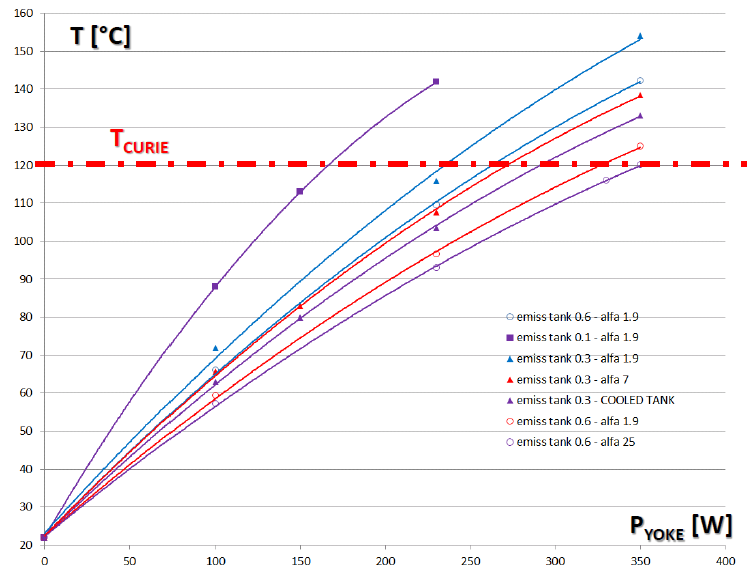
\includegraphics[width=0.8\textwidth]{LHC_MKI/figures/tempPowMarco.png}
\end{center}
\caption{The maximum steady-state temperature reached by the ferrite yoke in the MKI depending on the power load in the ferrite yoke as calculated using a 2D cross section of the MKI. $P_{yoke}$ is the power lost in the ferrite yoke and T the maximum steady state temperature of the ferrite yoke. Provided by M. Garlasche et al \cite{Garlasche:2dHeatEmisAll}.}
\label{fig:pow-loss-stable-temp-mkis}
\end{figure} 

Further monitoring of the MKIs will be necessary, as the stored current in the LHC is increased, due to possible further sources of heating within the magnets. However the work done on the understanding of the beam impedance, the heat transfer within the magnet and the electric field during kicker pulsing has greatly improved the knowledge of possible limitations in the future and the variety of solutions/counter measures that may be implemented. 